\chapter{Обзор предметной области}

В данной главе приведено описание предметной области. Описаны существующие подходы к алгоритмам ранжирования веб-страниц и стратегии приоритезации поискового робота.

\section{Основные понятия}

\subsection{Интернет как граф}
\label{webgraph}

Одной из формальных моделей, с помощью которой можно представить интернет, является его представление в виде направленного графа. Вершинами в этом графе являются веб-страницы, а ребрами --- ссылки. Из вершины $u$ есть ребро в вершину $v$, если на веб-странице, соответвующей узлу $u$ есть ссылка на веб-страницу, соответствующей вершине $v$. Заметим, что данный граф является динамическим, поскольку веб-страницы часто изменяются, какие-то из них удаляются, а также создаются новые. 

\subsection{Поисковая система}

Поисковая система --- это программный комплекс, предназначенный для помощи пользователю осуществления поиска информации в интернете. Основные компоненты поисковой системы представлены на рисунке \ref{poisk}. 

\begin{figure}[h!]
\center{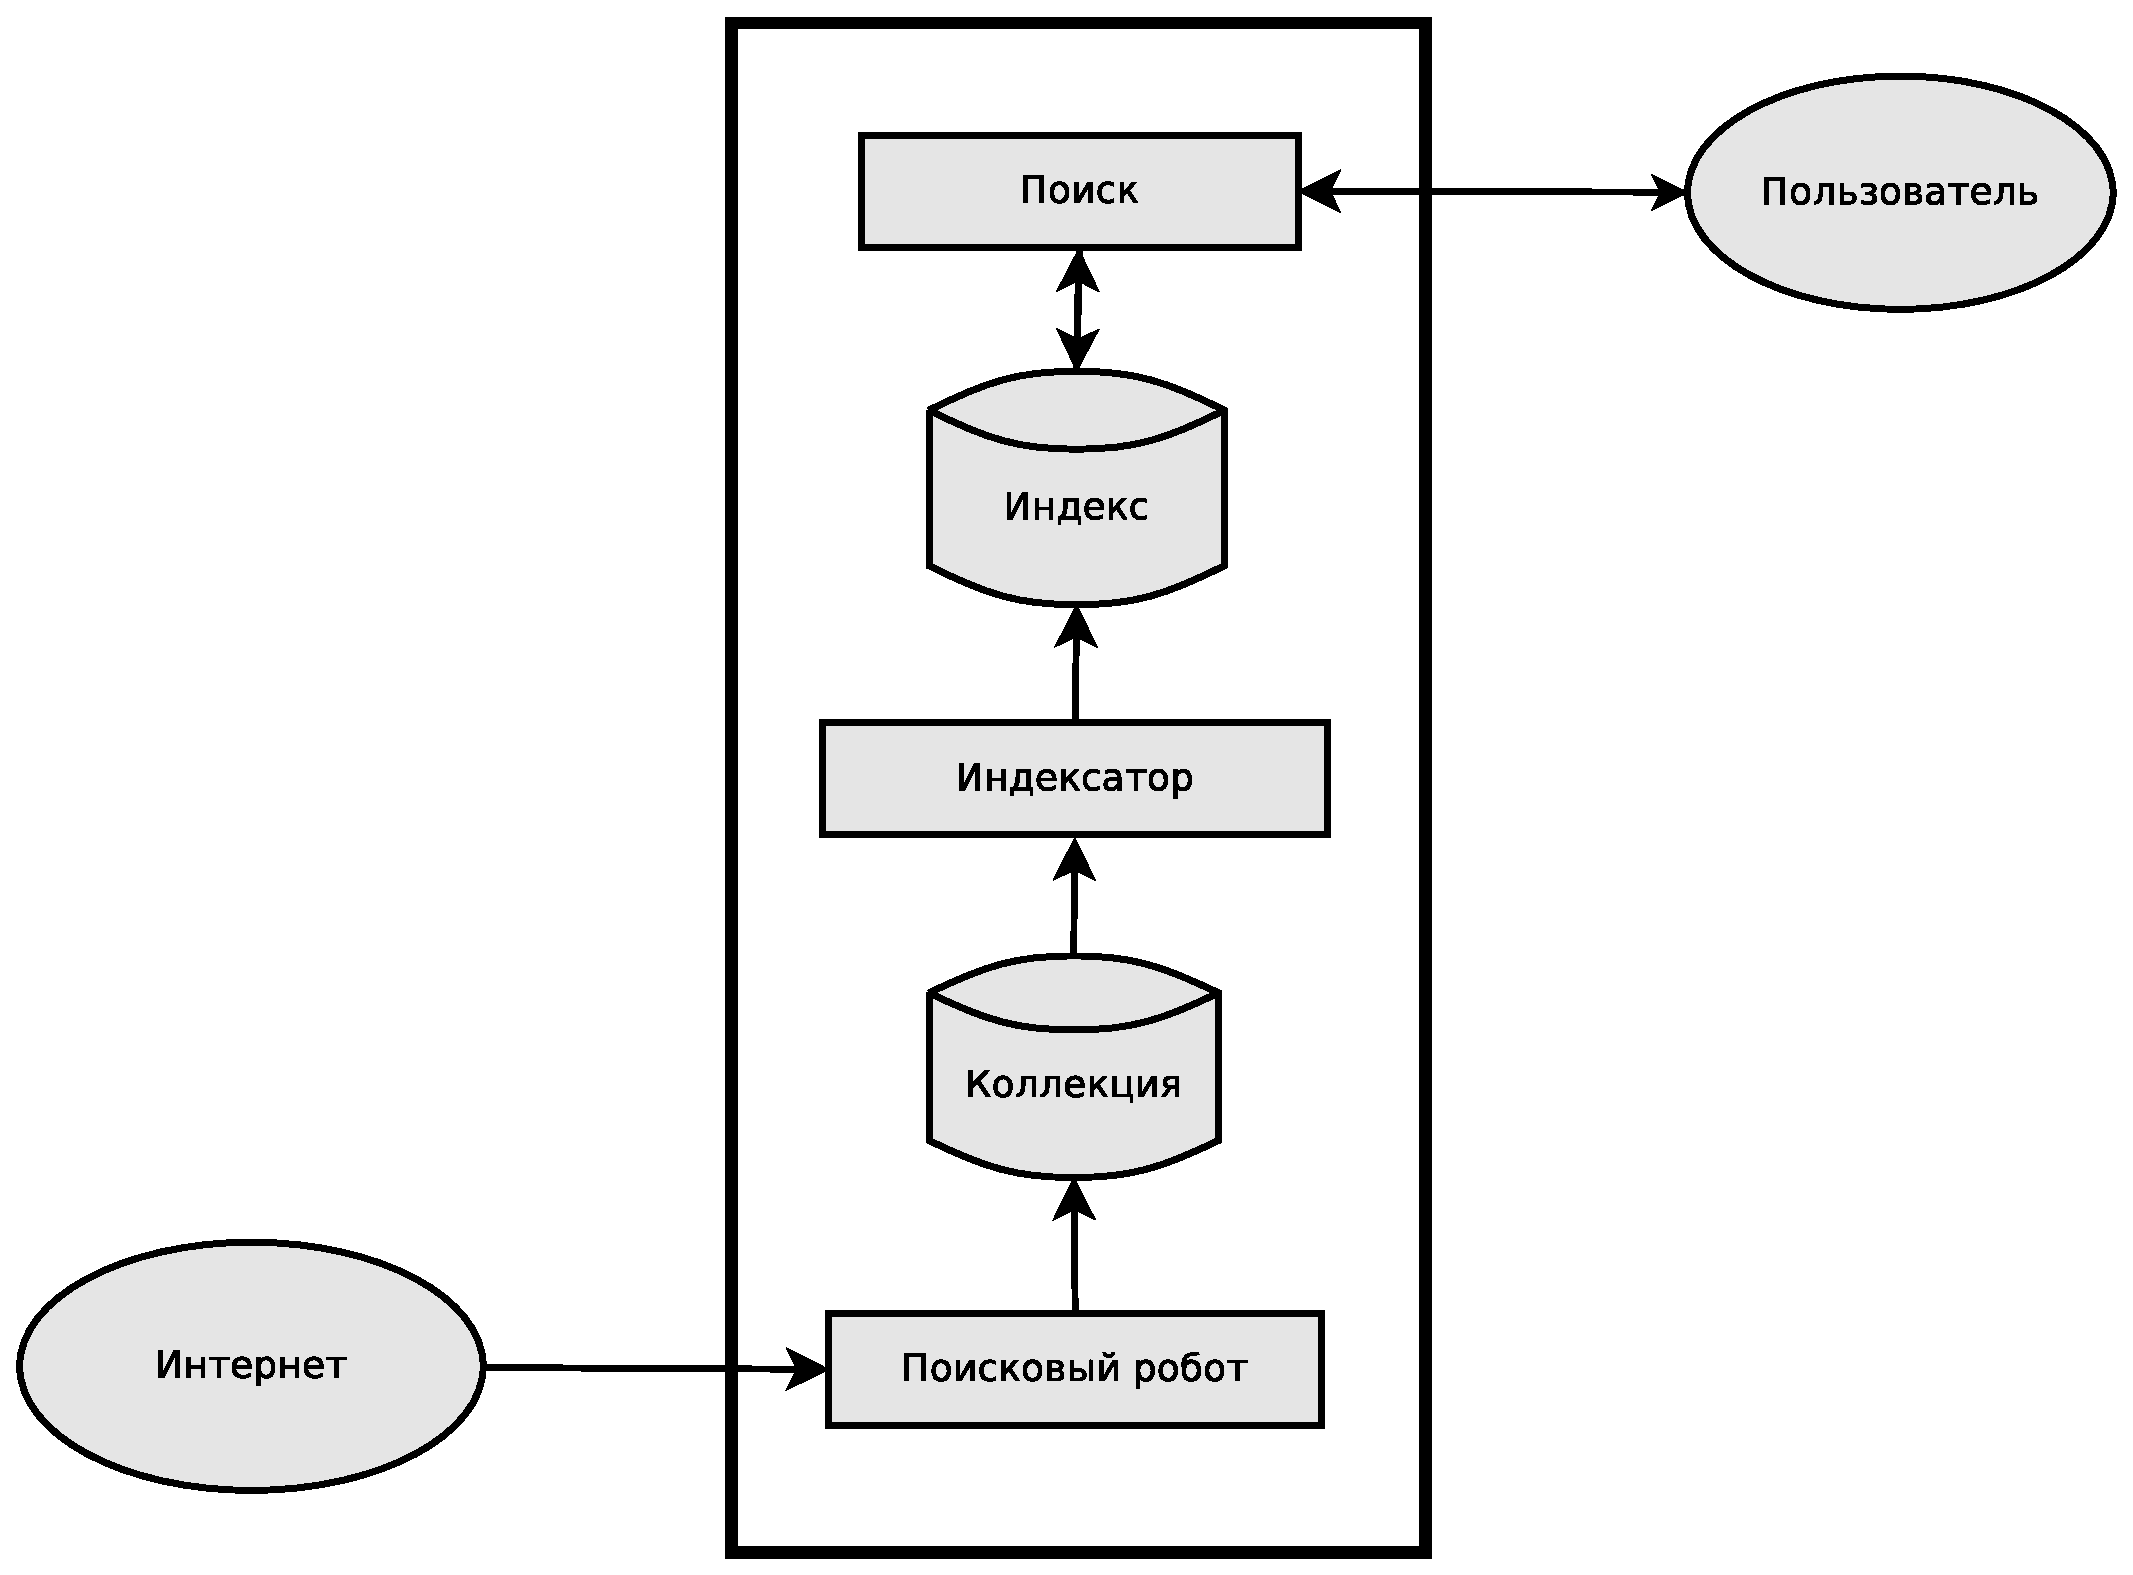
\includegraphics[width=1\linewidth]{pics/poisk.eps}}
\caption{Основные компоненты поисковой системы}
\label{poisk}
\end{figure}

Когда пользователь осуществляет информационный запрос, поисковая система формирует упорядоченное подмножество веб-страниц, хранящихся в ее индексе. Таким образом, качество работы поисковой системы во многом зависит от содержимого индекса, формирование которого осуществляется индексатором из множества веб-страниц коллекции, полученной в процессе обхода интернета, потому очень важно, чтобы в коллекции содержались важные веб-страницы, то есть веб-страницы, востребованные пользователем. Алгоритмы определения важности веб-страниц описаны в разделе \ref{ranking}. Коллекцию, в свою очередь, формирует поисковый робот. Подробное описание работы которого приведено в разделе \ref{spider}. Таким образом, поисковый робот в процессе обхода должен производить оценку страниц, и скачивать лишь важные. 

\section{Оценка важности веб-страниц}
\label{ranking}

Оценка важности веб-страницы называется рангом. Процесс получения оценки важности страницы называется ранжированием. Рассмотрим существующие методы, осуществляющие ранжирование.

\subsection{Алгоритмы ранжирования, использующие свойства веб-графа}

Данная категория алгоритмов использует представление интернета в виде графа, описанное в разделе \ref{webgraph}.

\subsubsection*{PageRank}

Метод разработан Сергеем Брином и Ларри Пейджом, основателями поисковой системы Google. Первая статья, описывающая этот алгоритм ранжирования была опубликована в 1998 году \cite{Brin}. Основная идея метода заключается в том, что страницы, чаще посещаемые в ходе случайного обхода веб-графа, имеют большую важность. 
Пусть имеется $N$ веб-страниц. Обход начинается с веб-страницы $p$, и в каждый момент времени с вероятностью $\alpha$ осуществляется переход по случайной ссылке, имеющейся на текущей странице. Также с вероятностью $1 - \alpha$ мы переходим на случайную страницу. Итоговая формула для вычисления PageRank имеет следующий вид: 
$$PageRank(p) = \frac{1 - \alpha}{N} + \alpha * \sum_{p' \in In(p)} \frac{PageRank(p')}{|Out(p')|}$$
где $In(p)$ --- множество страниц, содержащих ссылку на $p$, $Out(p')$ --- множество страниц, на которые ссылается $p'$, а $\alpha$ --- фиксированный параметр ($0 < \alpha < 1$). 

Ранжирование с использованием этого алгоритма является достаточно ресурсоемкой операцией, и требует знания о всей структуре веб-графа, что делает применение данного подхода на практике достаточно затруднительным.

\subsubsection*{HITS}

Hyperlink-Induced Topic Search (HITS) --- метод, разработанный в 1999 году Джоном Клейнбергом и описанный в работе. В отличие от \textit{PageRank}, является запросо-зависимым алгоритмом ранжирования, то есть полученные в результате анализа ссылок оценки веб-страниц зависят от конкретного поискового запроса. Базовая идея алгоритма заключается в том, что определенные веб-страницы являются \textit{посредниками} (\textit{hubs}), то есть используются как каталоги, указывающие на другие страницы, являющиеся авторитетными источниками (\textit{authorities}) или \textit{авторами} \cite{wiki_hits}, которые содержат необходимую пользователю информацию. Тогда страница, указывающая на большое количество хороших \textit{авторов}, является хорошим \textit{посредником}, и наоборот, страница, на которую ссылается много хороших \textit{посредников}, является хорошим \textit{автором}. Основываясь на этом, для каждой страницы вычисляется две оценки: оценка авторитетности и посредническая оценка. 

Для начала работы алгоритма необходимо получить множество наиболее релевантных страниц для текущего поискового запроса, называемое \textit{корневым множеством} (\textit{root set}). На его основе формируется \textit{базовое множество} (\textit{base set}), получаемое в результате добавления к \textit{корневому множеству} всех веб-страниц, связанных с ним ссылками, как исходящими, так и входящими. Все вычисления проводятся на подграфе, сформированном \textit{базовым множеством}. Основной алгоритм выполняет ряд итераций, на каждой из которых происходит обновление оценок для каждой вершины подграфа. Обновление посреднической оценки выполняется посредством суммирования оценок авторитетности каждой из вершин, на которые указывает текущая. В свою очередь, обновление авторитетной оценки осуществляется путем суммировния посреднических оценок вершин, ссылающихся на текущую. Окончательные оценки формируются после выполнения большого числа итераций алгоритма.

\subsection{Обучение ранжированию}
\label{learning_to_rank}

Алгоритмы данной категории используют методы машинного обучения для ранжирования документов. По обучающей выборке из элементов с заданным на них частичным порядком строится ранжирующая модель, которая затем используется для ранжирования новых данных. Как правило, необходимо отсортировать документы, отвечающие некоторому поисковому запросу. Элемент представляет собой пару: документ-запрос, для которой строится числовой вектор ранжирующих признаков. Признаки можно разделить на три группы:

\begin{itemize}
\item \textit{Запросо-независимые}. Зависят только от самого документа, а не от запроса. Например, \textit{PageRank} или длина документа.
\item \textit{Признаки запроса}. Зависят только от запроса. Например, число слов в запросе.
\item \textit{Запросо-зависимые}. Зависят как от документа, так и от запроса. Например, ранг \textit{HITS}, мера \textit{TF-IDF} соответствия запросу и т.д.
\end{itemize}

В статье \cite{Liu} рассмотрены существующие подходы к обучению ранжировнию и разделены на следующие категории в соответствии с форматом входных данных и функцией потерь:

\begin{itemize}
\item \textit{Поточечные подходы}. Каждому элементу сопоставляется численная оценка. Задача обучения --- по паре запрос-документ предсказать ее оценку. К ним относятся: \textit{OPRF, SLR, Pranking}.
\item \textit{Попарные подходы}. На вход подаются два документа и необходимо определить, какой из них лучше. Среди них алгоритмы: \textit{RankSVM, RankBoost, RankNet, FRank} и т.д.
\item \textit{Списочные подходы}. На вход подается сразу весь набор документов, соответвующих данному запросу, а на выходе должна получиться их перестановка. Среди них: \textit{ListNet, AdaRank, SoftRank, BayesRank} и т.д.
\end{itemize}

\section{Поисковый робот}
\label{spider}

\subsection{Общее описание}

Одним из важнейших условий функционирования поисковой системы является осуществление обхода интернета (web crawling). Его производит поисковый робот (web crawler or spider). Принцип его работы заключается в следующем. Робот хранит очередь URL-адресов веб-страниц, которые ему необходимо обойти. На момент начала обхода в ней находится некоторое исходное множество адресов. На каждой итерации робот извлекает из очереди следующий URL-адрес и скачивает веб-страницу, которая ему соответствует. Затем полученная страница обрабатывается, из нее извлекается содержимое и ссылки. Содержимое передается индексатору для последующей обработки и добавления страницы в базу поисковой системы. А URL-адреса страниц, содержащихся в ссылках, извлеченных с текущей страницы, добавляются в очередь на скачивание.

В книге \cite{Manning} сформулированы основные свойства поискового робота. Они разделены на две категории: обязательные и желательные.

\subsection{Обязательные свойства}

Обязательными свойствами поискового робота являются:
\begin{enumerate}
\item Устойчивость. 
\item Вежливость. 
\end{enumerate}

Остановимся на каждом из них подробнее.

\subsubsection*{Устойчивость}

Число страниц в интернете потециально может быть бесконечно, поскольку некоторые веб-сервера генерируют динамические веб-страницы по запросу на их создание, которым, в частности, является переход по ссылке. Таким образом, поисковый робот может зациклиться на определенном хосте, бесконечно скачивая вновь сгенерированные динамические страницы. Такой механизм называется ловушкой для роботов (spider trap). Поисковый робот должен быть устойчив к подобного рода явлениям.

\subsubsection*{Вежливость}

Для сайтов существуют явные и неявные правила поведения поискового робота при работе с ними. Эти правила регулируют частоту обращения к хосту, а также возможность доступа к его содержимому. Многие сайты имеют в корне специальный файл $robots.txt$, содержащий желательные правила поведения. Поисковый робот должен соблюдать их.

\subsection{Желательные свойства}

Желательными свойствами поискового робота являются:

\begin{enumerate}
\item Распределенность.
\item Масштабируемость.
\item Производительность и эффективность.
\item Качество.
\item Свежесть.
\item Расширяемость.
\end{enumerate}

Остановимся на каждом из них подробнее.

\subsubsection*{Распределенность}

Подразумевает возможность функционирования поискового робота одновременно на многих машинах.

\subsubsection*{Масштабируемость}

Подразумевает возможность увеличения эффективности поискового робота при увеличении ресурсов. Таких как увеличение числа машин или расширения полосы пропускания.

\subsubsection*{Производительность и эффективность}

Подразумевает эффективное использование поисковым роботом доступных ему ресурсов. 

\subsubsection*{Качество}

Желательно, чтобы поисковый робот при скачивании веб-страниц отдавал предпочтение более качественным. Для выполнения этого свойства необходима стратегия приоритезации страниц. Существующие стратегии подробнее рассмотрены в разделе \ref{algorithms}.

\subsubsection*{Свежесть}

Для хранения свежей информации о веб-страницах в базе поисковой системы необходимо, чтобы поисковый робот обходил ранее скачанные страницы с частотой, соответствующей частоте их обновления. Способы выполнения этого свойства также рассмотрены в разделе \ref{algorithms}.

\subsubsection*{Расширяемость}

Поисковый робот должен быть разработан так, чтобы имелась возможность расширения для решения новых задач. Таких как добавление новых протоколов передачи данных или новых форматов данных. 

\section{Алгоритм приоритезации поискового робота}
\label{algorithms}

Под приоритезацией подразумевается введение полного или частичного порядка на множестве веб-страниц, которое поисковый робот должен обработать. Это необходимо для того, чтобы поисковая система хранила в базе страницы, содержащие информацию, которая необходима пользователю, осуществяляющему поисковый запрос. Скачивание качественных веб-страниц осуществляется за счет применения стратегии отбора, а наличие свежей информации в базе данных поисковой системы осуществляется за счет применения той или иной стратегии повторного обхода. Объединение этих двух стратегий составляет стратегию приоритезации поискового робота. 

\subsection{Стратегии отбора}
\label{selection_strategy}

Стратегия отбора определяет, в каком порядке поисковый робот должен обрабатывать веб-страницы, URL-адреса которых были добавлены в очередь на скачивание. Для этого необходимо осуществить эвристическую оценку важности для каждой веб-страницы, являющейся кандидатом на скачивание. В книге \cite{Castillo} стратегии отбора разделены на три категории, описанные ниже.

\subsubsection*{Стратегии, не использующие дополнительную информацию}

Стратегии, отнесенные в данную категорию, используют информацию, полученную в процессе текущего обхода, и никакую более.

\textbf{Обход в ширину}. При использовании данной стратегии поисковый робот скачивает новые страницы, осуществляя обход в ширину веб-графа, начиная с главных страниц стартового множества. То есть веб-страница будет скачана тем раньше, чем раньше ссылка на нее была извлечена с какой-либо скачанной веб-страницы. В работе \cite{Najork} показано, что в проведенных экспериментах поисковый робот, использующий данную стратегию, выбирал важные страницы первыми.

\textbf{OPIC}. Данный метод описан в работе \cite{OPIC}. Этот метод также базируется на представлении веба как графа, описанному в разделе \ref{webgraph}. В начале обхода каждой странице присваивается одинаковая стоимость. После загрузки страницы ее стоимость поровну распределяется между веб-страницами, на которые она ссылается. Более высокий приоритет имеют страницы с высокой текущей стоимостью. Вычисление стоимости аппроксимирует вычисление \textit{PageRank}. 

\textbf{Количество обратных ссылок}. Данная стратегия была описана в работе \cite{Cho2}. В этом алгоритме первыми скачиваются страницы, имеющие наибольшее число входящих ссылок.

\textbf{FICA}. Метод подробно описан в статье \cite{FICA}. Алгоритм базируется на методике обучения с подкреплением, где для каждого узла веб-графа вычисляется ранг на основании расстояния между страницами.

\subsubsection*{Стратегии, использующие информацию, полученную ранее}

Стратегии данной категории используют информацию о рангах страниц, полученную в результате предыдущих обходов. При этом поисковый робот начинает обход со страниц, имеющих более высокий ранг, а ранги для страниц, найденных впервые, рассчитываются следующими способами: 

\begin{itemize}
\item Запрашивая информацию о рангах у <<оракула>>, располгающего полной информацией о веб-графе;
\item Равновероятно выбирая одно из значений рангов страниц, полученных в предыдущих обходах;
\item Назначаются нулем, то есть сначала скачиваются все страницы, известные ранее, а затем --- новые;
\item Как значение ранга страницы, указывающей на нее, деленное на число ее исходящих ссылок.
\end{itemize}

По результатам экспериментов в работе \cite{Castillo}, стратегии данной категории преимущественно превосходят стратегии, не использующие дополнительной информации. При этом лучшим является метод, запрашивающий информацию о рангах у <<оракула>>.

\subsubsection*{Стратегия с полной информацией}

К данной категории относится одна стратегия \textit{Omniscient}, использование которой подразумевает наличие <<оракула>>, который вычисляет актуальный ранг для каждой веб-страницы. Для того, чтобы выбрать страницы из очереди на скачивание, поисковый робот осуществляет запрос к <<оракулу>>, после чего выбирает страницы с наибольшим рангом. Данная стратегия быстрее всего находит важные страницы.
 
\subsection{Стратегии повторного обхода}

Стратегия повторного обхода определяет какие из уже скачанных страниц следует скачать еще раз. Оба типа стратегий описаны в работе \cite{Cho}:

\begin{itemize}
\item \textit{С одинаковой частотой}. Данная стратегия подразумевает, что веб-страницы будут скачиваться с одинаковой частотой, при этом их важность никак не будет учитываться.
\item \textit{С разными частотами}. При использовании данного типа стратегии, веб-страницы скачиваются с разными частотами. Например, с частотами, пропорциональными частотам изменения страниц.
\end{itemize}
